\documentclass[]{revtex4-2}
\usepackage{siunitx}
\usepackage{graphicx}

\begin{document}

\title{Improving Nb\textsubscript{3}Sn Cavity Performance Using Centrifugal Barrel Polishing}
\author{Eric Viklund}
\email{ericviklund2023@u.northwestern.edu}
\affiliation{Department of Materials Science and Engineering, Northwestern University}
\affiliation{Fermi National Accelerator Laboratory}
\author{David N. Seidman}
\affiliation{Department of Materials Science and Engineering, Northwestern University}
\author{Sam Posen}
\email{sposen@fnal.gov}
\affiliation{Fermi National Accelerator Laboratory}


\date{\today}

\begin{abstract}

    Despite having superior superconducting properties, Nb\textsubscript{3}Sn SRF cavities are still impractical in many ways compared to Nb SRF cavities due to the brittle nature of Nb\textsubscript{3}Sn. One major concern is the performance degradation that can occur when a Nb\textsubscript{3}Sn experiences mechanical stresses such as during handling and tuning of the cavity. In this study we present a potential treatment for cavities that have experienced stress induced performance degradation that involves a recoating procedure. During this procedure, the degraded cavity is coated with a small amount of tin using the vapor-diffusion method. Using this procedure we are able to recover a significant portion of the lost performance of a Nb\textsubscript{3}Sn SRF cavity.

\end{abstract}

\maketitle

\section{Introduction}
\label{sec:Introduction}

A higher T\textsubscript{c} makes Nb\textsubscript{3}Sn an attractive material for SRF applications. However, the material properties of Nb\textsubscript{3}Sn make it difficult to work with. The brittleness of the material introduces new challenges to the cavity manufacturing process. Particularly for handling and tuning of the cavity, which can induce stresses on the cavity. Nb\textsubscript{3}Sn cavity performance is known to degrade severly when stresses are applied to the cavity. This degradation is theorized to be caused by cracks in the brittle Nb\textsubscript{3}Sn film. Cavities that suffer from degradation must be stripped and recoated with a new Nb\textsubscript{3}Sn film, which is a time consuming and expensive process.

In this study we will explore a new procedure to heal Nb\textsubscript{3}Sn cavities that have been degraded. This procedure utilizes a short Nb\textsubscript{3}Sn recoating to heal cracks that have formed in the cavity without the need to remove the original film. Using this procedure, we are able to recover a large portion of the performance of a degraded Nb\textsubscript{3}Sn cavity with just a simple procedure.

\section{Experiment}
\label{sec:Experiment}

The cavity was coated using high-temperature nucleation step to create a low roughness Nb\textsubscript{3}Sn film. An in-depth analysis of this cavity coating and initial performance was published by Posen et. al.~\cite{posen2021advances}. 

After testing the performance of the cavity, the cavity was damaged during transport leading to a sharp decrease in the performance. We theorize that the degradation was caused by stresses applied to the cavity during transport, which led to the formation of cracks. This type of performance degradation has previously been observed when tuning Nb\textsubscript{3}Sn cavities at room temperature~\cite{eremeev:srf2019-mop015}, which indicates that both situations are caused by stress induced cracks in the film.

To heal the damage caused to the cavity, we apply a recoating procedure. For the recoating procedure, the cavity was heated to \qty{1000}{\degreeCelsius} and exposed to Sn vapor for \qty{1}{\hour}. Sn vapor was provided by \qty{0.85}{\gram} of Sn heated to \qty{1250}{\degreeCelsius}.

\section{Result}
\label{sec:Results}

The performance of the cavity after the initial coating was stellar, reaching a peak accelerating field of 24~MV/m and maximum Q of \num{2e10} at \qty{4}{\kelvin}. After the cavity was damaged the performance was severly degraded. The cavity only reached \qty{8}{\mega\volt\per\meter} and a slight decrease in quality factor.

\begin{figure}[h!]%
    \centering%
    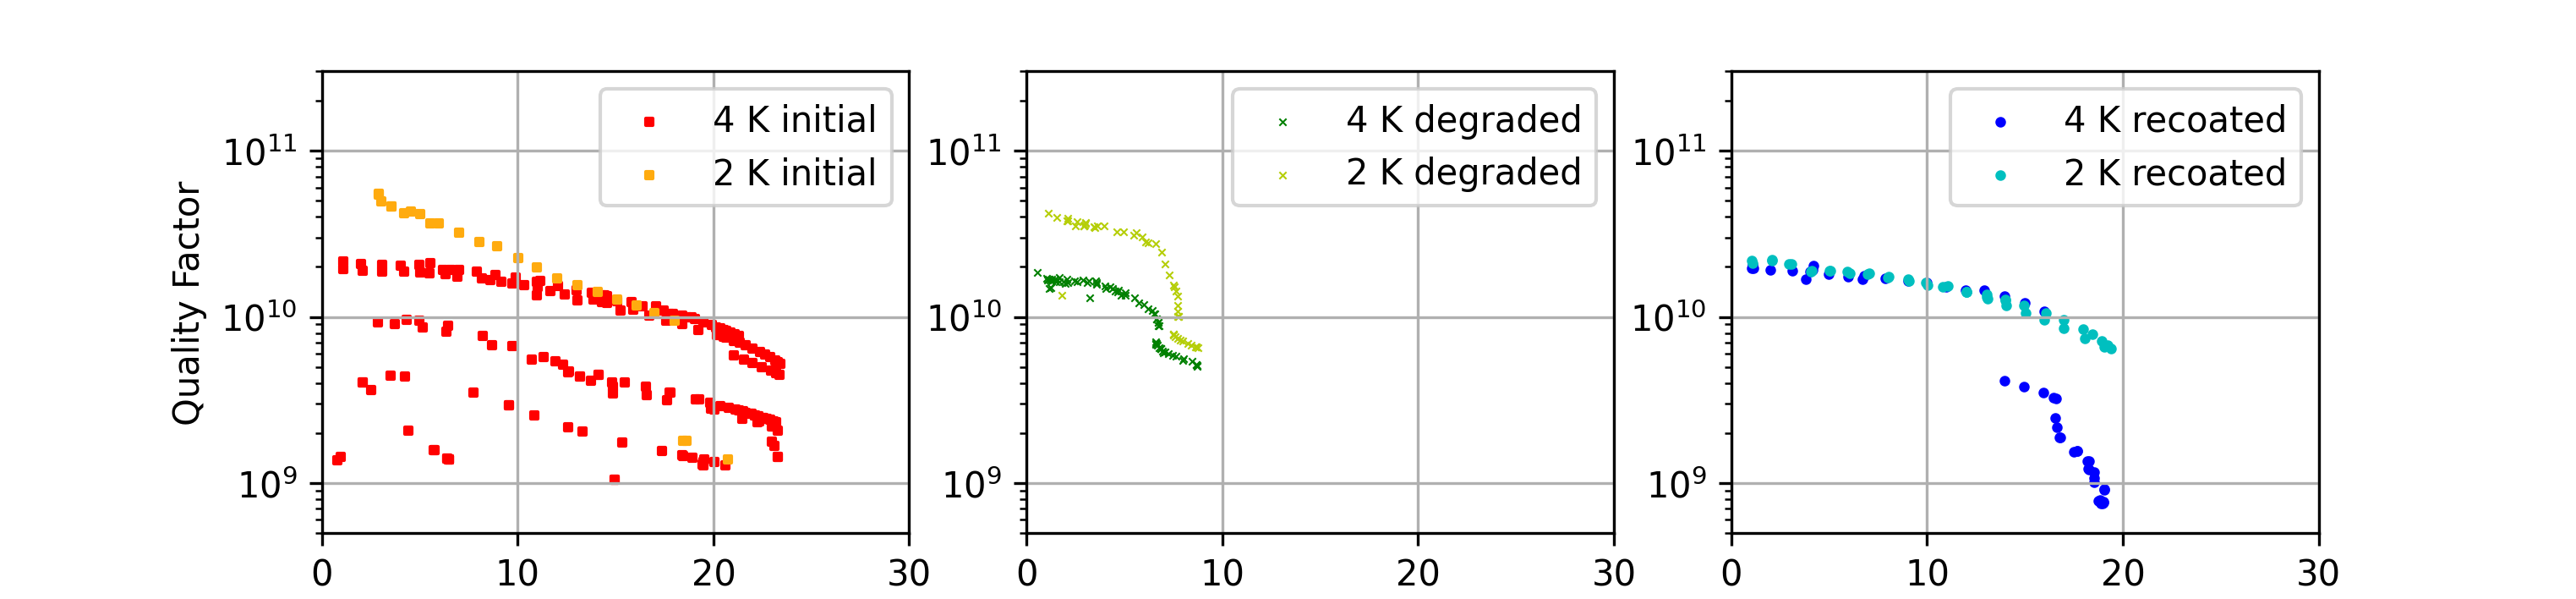
\includegraphics[width=1.0\columnwidth]{./figures/VTS.png}%
    \caption{}%
    \label{fig:VTS}%
\end{figure}

Temperature mapping was used to locate the quench source. A single hot spot on the equator of the cavity was discovered. Visual inspection of the cavity showed no visible defects near the quench location indicating that the defect must be microscopic.

After the recoating was applied the cavity saw a significant increase in performance. The peak accelerating gradient increased to \qty{18}{\mega\volt\per\meter} and the quality factor also increased to \num{3e10} at \qty{4}{\kelvin}. This indicates that the quench causing defect has been repaired. 

Temperature mapping of the cavity after recoating shows







\begin{figure}[h!]%
    \centering%
    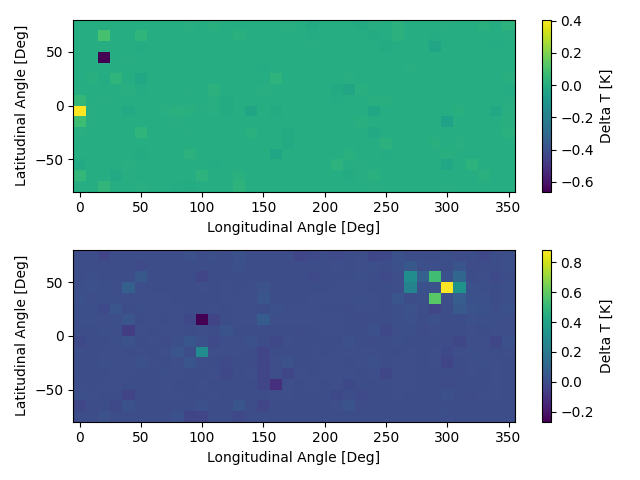
\includegraphics{./figures/TMAP.png}%
    \caption{}%
    \label{fig:VTS}%
\end{figure}


\section{Discussion}
\label{sec:Discussion}

Using a low temperature Sn recoating process, we were able to heal a degraded Nb\textsubscript{3}Sn cavity that has suffered damage during transportation. This discovery provides a new tool that can be applied to similarly degraded cavities to recover some performance. This will save time and money that would otherwise be spent by stripping the Nb\textsubscript{3}Sn coating and applying a new coating. This process could make Nb\textsubscript{3}Sn cavities more viable for real-world accelerator applications by reducing the cost of manufacturing and transportation errors.



\bibliographystyle{plain}
\bibliography{bib}

\end{document}